\thepage
\section{Introduction}

%- No collocation
%- Enterprise support
%- Version control, issue tracking

In recent years open source software solutions have become widely popular and frequently used in both scientific and enterprise use, which can be attributed to a number of factors, most importantly the ease of development and deployment of IT projects, improved cybersecurity and enhanced scalability \cite{pwcLeadingBenefitsOpensource2016}. This increases the contribution to open source projects from enterprises and individuals alike. Due to its nature, open source software projects are driven by community contributions, and depend heavily on active participation in all phases of the project. \\

Software development in a corporate environment usually follows a strict hierarchial structure, where each participant is given a precise position and responsibility, like project manager, scrum master, senior or junior developer, and employees do not tend to work outside of their assigned tasks and territories. The main purpose of maintaining software development structures is for the company to ensure that the outcome of the project is in accordance with the business objective, adheres to the pre-set quality criteria and it is completed in a given timeframe; in other words to asses the risks associated with the business objective of the software project \cite{surekaUsingSocialNetwork2011}. This is achieved by breaking down the developed software into smaller, less complex components, and grouping the developers into managable teams, where the communication is moderated between teams \cite{birdLatentSocialStructure2008}. \\

% Open-source software development propertie
As opposed to commercial software development, Free/Libre Open Source Software (FLOSS) projects usually do not follow an organizational hierarchy, and are usually self-organizing and dynamic \cite{birdLatentSocialStructure2008}. Issues, bugs and progress are tracked openly, and everyone is encouraged to contribute based on the current topics and expertise, but purely on a volunteering basis. The lack of access restriction to certain modules allows for much more spontaneous interaction between developers, which generate large, complex networks \cite{martinez-romoUsingSocialNetwork2008}. These complex networks can be seen as large social networks of developers based on collaboration. \\

% AUTHOR NAME HARDCODED HERE
Because contribution to FLOSS projects are voluntary, participants have a different motivation for taking part than in commercial software development. According to El Asir et al. \cite{elasriPeripheryCoreTemporal2017}, FLOSS participation can be motivated by internal and external factors. Internal factors include self-improvement, learning and contribution as a hobby or pass-time activity  \cite{alexanderharsWorkingFreeMotivations2002,yunwenyeUnderstandingMotivationOpen2003}, whereas external factors are motivated by marketing and demonstrating certain skills, thus increasing and improving employability \cite{alexanderharsWorkingFreeMotivations2002}. \\

% Summary of background literature and state of the art solutions
\section{Background and rationale}

\subsection{Collaboration in FLOSS projects}
% - FLOSS definition
% AUTHOR NAME HARDCODED HERE
Collaboration networks of open source software (OSS) have been a subject of many academic research. Raymond \cite{crowstonSocialStructureFree2005} has defined collaboration based on bug report interaction, and observed the collaboration network of 124 large-scale SourceForge projects. The generated networks have widely different centralization properties, but it was observed that larger sized projects tend to be more decentralized. The broad community roles contributors tend to take have been also identified in \cite{crowstonSocialStructureFree2005}, which have been coined as the \textit{onion model} in \cite{martinez-romoUsingSocialNetwork2008} (Figure \ref{fig:onion1}). \\

\begin{figure}
    \centering
    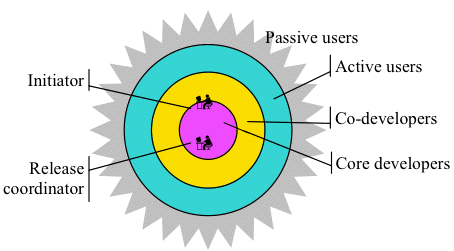
\includegraphics[width=0.6\textwidth]{figures/onion_model.png}
    \caption{Onion model of collaboration types in FLOSS projects \cite{crowstonSocialStructureFree2005}.}
    \label{fig:onion1}
\end{figure}

The onion model describes the types of participants in an OSS project as layers. The center represents the small group of core developers, who are responsible for the majority of contributions to the software. They are surrounded by a larger group of co-developers, whose main contributions are usually bug fixes reported by the active users. The passive users are usually the largest in numbers, who do not contribute or report any bugs. In a healthy FLOSS project, each layer of contributors are about one magnitude larger in numbers than the preceeding inner layer \cite{mockusTwoCaseStudies2002}. \\

% AUTHOR NAME HARDCODED HERE
El Asir et al. \cite{elasriPeripheryCoreTemporal2017} used a K-means classification to categorise project participants into a similar core-periphery structure (core, gray in-between area, and periphery) based on SNA metrics with a montly timeframe, and analysed how and why contributors transition between groups. They found that technical contributions like code commits and lines added have a much heavier impact on becoming a core developer as opposed to other activities, such as testing, reviewing and commenting. \\

% AUTHOR NAME HARDCODED HERE
A literature review conducted by McClean et al. \cite{mccleanSocialNetworkAnalysis2021} systematically analysed the state-of-the-art research of 46 scientific papers in the field of FLOSS social networks, and categorised them into three groups based on topic: structure, lifecycle and communication. They conclude, that the existence of core-periphery structure in OSS projects is well established in the field, which is also an indicator of a healthy FLOSS software. Regarding the lifecycle, generally the core development team does not change significantly over time, however, the project becomes more decentralised and distributed as it matures. A lack of research regarding temporal analyses were identified in the most current knowledge, which was suggested as a future research area in this field. \\

\subsection{Social network of Open-source projects}
In a larger FLOSS project, developers usually cannot understand every part of the project, therefore collaboration is required with eachother. The network created by the collaborators can be considered as a social network, because collaboration requires some kind of social interaction with eachother. Social network theory describes how social interaction patterns affect the individual behaviour \cite{martinez-torresGeneticSearchPatterns2012}. We can model an OSS project's social network as a graph, where nodes represent collaborators (developers, bug reporters, etc\dots) and edges represent the social interaction between them. In mathematical terms\dots \\

The type of the social interaction determines the created network, therefore choosing the basis of collaboration can have a significant impact on the network structure. The common types of developer social networks (DSNs) are Version Control System-based (VCS-DSN), Bug Tracking System-based (BTS-DSN) networks and DNSs, that are purely based on social elements \cite{aljemabiEmpiricalStudyEvolution2018}. The VCS-DSN take the version control application as a source for network generation by recording collaboration based on co-edits of the same module, file or code section. Choosing the granularity can impact the precision of true collaborations represented in the network. Co-edits by multiple developers to a single module or file does not necessarily mean actual collaboration was required from the authors, as the parts edited could work functionally independent from eachother. By increasing the granularity to file sections (classes or functions within a single file) or even lines, we can be more certain, that coordination was required, but we risk leaving out semantically connected parts of the project \cite{joblinEvolutionaryTrendsDeveloper2017}. In contrast to VCS-DSNs' purely technical approach, the BTS-DSNs use semi-technical bases for connecting participants, such as comments on issues, bugs or reviews \cite{elasriPeripheryCoreTemporal2017}. These artifacts, although being tightly related to specific sections of the source code, allow for taking into account conversational elements as contribution. For example, participants, who do not contribute directly to the software source code, but actively review and comment, are also considered. Lastly, social networks of developers can be constructed on project participation, following, starring or through communication means like mailing lists. The technical aspect of collaboration is minimized in such DNSs, and they are more fit for project organization and communication analyses in FLOSS projects (mailing list vs file file edits vs line edits) \\


% \subsubsection{Global SNA metrics}

% \subsubsection{Local SNA metrics}

%\begin{itemize}
%   \item Relevant social aspects of OS projects
%   \item State of the art
%   \item Collaboration by coediting files
%   \item Contributors form dynamic social networks
%    \item Problem of analysing changes over time in a network
%   \item Other studies in this field...
%\end{itemize}

\subsection{OSS project success}
community maturity (\cite{linBlogCommunityDiscovery2007} in \cite{aljemabiEmpiricalStudyEvolution2018}) \\

"Successful projects will likely have modular structure from the start or after refactoring as the source code grows larger and more unwieldy" \cite{antwerpEvolutionOpenSource2010} \\

success factors: Average Time Efforts, Number of Developers, Comments, Total Code Lines, Comment Ratio, Number of Rater \cite{yangHowMicrobloggingNetworks2013}
Truck Factor \cite{avelinoNovelApproachEstimating2016}


\section{Motivation of research problem and research questions}
Because there is a high dependency on the community in open source software projects, by understanding how contributions are included and what patterns emerge we can gain valuable insight into the project's current state and its trajectory. As stated before, SNA analysis of OSS have been extensively studied, but there is a lack of research regarding temporal models analyzing the lifecycle of a FLOSS project. \\

The goal of this paper is to fill in this gap by examining OSS project collaboration networks over time using SNA metrics. More specifically, one part of the research will focus on the evolution of such collaboration networks and comparing and contrasting these networks with the software outcome. The second part will focus on events during a project, and how it affects the developer collaboration. The research questions, which are broken down into subquestions, are as follows:

\begin{enumerate}
    \item \textbf{How does the temporal lifecycle information of a project influence its success?} \\
    
    \begin{enumerate}
        \item \textit{Based on temporal models of collaboration, is it possible to predict the outcome of the project?} Since it has been proven that the core collaborators do not change much over the course of the OS software development, our assumption is that any sudden or long-term change, that is not consistent with the other observed projects, can have a significant impact on the outcome (negative or positive alike).
        \item \textit{Can stages of a FLOSS project with a maturity model be observed?} As most OS software starts with a small collaborator basis and grows over time, it can be assumed, that each project goes through the same steps of open source maturity levels. On the other hand, it is also possible that due to the uniqueness of each project, no such stages are observable. 
    \end{enumerate}

    \item \textbf{How do major events in the project lifecycle change the collaboration network of the project?}
    \begin{enumerate}
        \item \textit{Do planned or foreseeable events change the collaboration structure?} Major software version releases can be considered foreseeable events of the project lifecycle, which could have an effect on the developer collaboration. For example, there might be a higher rate of interaction between contributors just before a new version is released to clear up the backlog of tasks. But it is also possible, that commit and change rates drop during this time, because the focus shifts to stability and testing instead of new features.
        \item \textit{How unforeseeable internal or external events affect FLOSS collaboration?} Sudden shocks to the project, such as an announcement of disinterest from major users of the software, discontinued enterprise support of the project, large-scale global events like the pandemic, or sudden employee firings can have significant effect on the core and periphery collaborators alike. By analysing the collaboration network before, during and after such changes, we might be able to recognise patterns, that regularly occur around these events.
    \end{enumerate}
\end{enumerate}

\subsection{Research methodology}
To find answers to the research questions above, first we build a repository analyzer tool, which mines collaboration data from FLOSS projects, generates static snapshot collaboration networks at each given time interval and calculates SNA metrics for each snapshot. Then these metrics can be aggregated over time, or plotted against time to discover changes in the network. The \texttt{git2net}\footnote{\url{https://github.com/gotec/git2net}} \cite{goteAnalysingTimeStampedCoEditing2019} Python library provides the necessary tools to mine any project repository that uses git version control. It also incorporates temporal network generation capability, which can be used as a source for creating static collaboration networks aggregated over a given period of time. \\


We apply a hybrid methodology of qualitative and quantitative research. First, as part of the qualitative research, we choose a small number of repositories to be analyzed. We observe the number of connected components, centrality, number of nodes and mean degree SNA metrics in order to discover the core and peripherial collaborators over the project lifecycles. The basis of collaboration, due to the unavailability of other means of communication, is coediting files. Based on the state of the art research in this field, file coediting proves to be an effective and easy way to represent collaboration between developers. \\

After discovering the collaboration structure over time, we will match the breakpoints and unexpected spikes or troughs to events within the lifespan of the project. We expect that the key SNA metrics will show a periodicity around planned releases and other reoccurring events (e.g. holiday season). Outstanding values without reoccurrence, on the other hand, are more likely to be consequences of unexpected events. In these cases, it should be observed whether the network is capable of reorganizing itself, or does the event leave a permanent mark on the collaboration structure. A categorization of unexpected events and the level of impact each category has should be observed. \\

For the quantitative research to be conducted, we will gather a large set of repositories along with major events in its lifecycles. We will then run the miner for all repositories, and with the findings of the qualitative research, we will try to detect all major events and their type (planned or unexpected). We will utilize the \texttt{ruptures} \footnote{\url{https://github.com/deepcharles/ruptures}} library to detect changes in the continuous SNA metrics. If the model is capable to accurately recognise events, then we can also apply it on any repository to detect changes, which will allow us to discover changes in the collaboration network that are not related to publicly known events or releases. \\

% Quantitative research
% \begin{itemize}
%     \item Composing a large set of repositories (different sizes, properties) with their success or failure
%     \item Gathering major events for the repositories (version releases, external events, global events)
%     \item Detecting past changes automatically based on changes in measured statistics
%     \item How do changes and reoccurring patterns match the events?
%     \item What structures can be noticed before a major success or failure of a project?
% \end{itemize}


\section{Gitminer implementation}
To find answers to the research questions, we implement an analysis tool to mine and analyze project repositories, which allows us to generate collaboration networks and network metrics for the analysed projects. \\

\subsection{\texttt{git2net} miner}
The process begins with the project mining. After cloning the repository, the \texttt{git2net} \cite{goteAnalysingTimeStampedCoEditing2019} library is used to collect data related to commits. Specifically, who is the author of each commit, which files were modified (created, edited, deleted) with the commit, and when was the commit created. Additionally, the lines edited by the author within each commit are collected separately, allowing for a more fine-grained collaboration network generation if necessary. The results are collected into an \texttt{sqlite} \footnote{\url{https://www.sqlite.org/index.html}} database file's \textit{commits} and \textit{edits} tables. \\

The \texttt{git2net} mining process by default collects all the commits throughout the project's lifecycle. However, the processing time of each commit differs based on the number of edits, the affected number of files and the file types as well, which makes collecting certain commits very resource-intense and time-costly. Therefore, we exclude every commit, which contains more than 100 file modifications, during each repository mining using the \textit{max\_modifications} parameter. As observed by Gote et al \cite{goteAnalysingTimeStampedCoEditing2019}, this exclusion criteria does not affect significanly the generated network, because they are mostly merge commits or project restructurings, which do not mark any true collaboration effort between developers. During the data mining in certain repositories, we encountered commits, that were not mineable with this method and the mining process halted, presumably due to processing error because of binary file changes in these commits. We also excluded these commits from our data mining process.\\

This exclusion criteria resulted in an average of 3\% of commits excluded in all repositories subject to our analyses, with the highest excluded commit rate being 20\%.

\subsection{\texttt{repo\_tools} miner} 

We use the \texttt{repo\_tools} \footnote{\url{https://github.com/wschuell/repo\_tools/}} Python library to query the Github API for additional repository data extraction, such as:

\begin{itemize}
    \item Releases
    \item Tags
    \item Issues
    \item Stars and followers
\end{itemize}

The mining output is also stored in a \texttt{sqlite} relational database, which is queried later on during the analysis. 

% - what do we want to achieve with the gitminer
%  - generate networks of collaboration
%    - what should be the basis of collaboration
%  - filter for time
%  - generate statistics

\subsection{Data preprocessing}

The collaboration networks with the \texttt{git2net} library connect the authors to their edited files using only file and author names instead of IDs. This creates an issue when generating the networks, because authors with the same name will show up as one node, and they will be connected to the files they touched combined. Furthermore, authors that change their displayed name ('author\_name' field in the mining database) or log in from diferent accounts, where they have different names, will show up as multiple nodes instead of a single vertex. \\

We utilize the \texttt{gambit} \cite{goteGambitOpenSource2021} rule-based disambiguation tool to resolve the author names. Furthermore, the created networks have issues when the node names contain special characters or spaces. Therefore, after disambiguation, we replace every unique author name with its ID number. \\

As the files are also labelled by their filename property in the network outputs, the same filenames but in different folders are also displayed as single nodes. In order not to create false collaborations, we simply remove the files from the network with filenames, that occur more than once in all the repository subdirectories. We argue that this does not remove any significant collaboration data, since most files sharing their name with other files are technicaly files, like \texttt{\_\_init\_\_.py} for a Python project. \\

\subsection{Collaboration networks}

When creating a DSN from the mined data, we have multiple methods at hand. The \texttt{git2net} library provides its own co-editing network function, which returns a temporal network of collaborators. This uses the co-authorship algorithm developed by Gote et. al. \cite{goteAnalysingTimeStampedCoEditing2019}, however, we would like to have more control over the network generation method, such as simple file-based co-authorship in order to customize the network for our needs, like weighing each relation or generating undirected graphs. \\

\subsubsection{Temporal bipartite network}
As a first step, we generate a temporal bipartite network of authors and their edited files with the \texttt{git2net} built-in \textit{get\_bipartite\_network} method. A temporal network is a \texttt{pathpy} \footnote{\url{https://www.pathpy.net/}} graph object, which contains a collection of timestamped graphs of a single network at each point in time within the observed timeframe. Such a snapshot $S_t = (U, V, E_t)$, where $U$ is the set of authors, $V$ is the set of files and $E_t$ is the set of file edits as edges at $t$ timestamp. By connecting the authors, who touched the same files, and removing the nodes representing the edited files (converting the bipartite network to a regular network), we can observe the evolution of the collaboration over time, represented in Figure \ref{fig:temporal net}. \\

\begin{figure}
    \centering
    \begin{subfigure}{0.3\textwidth}
        \centering
        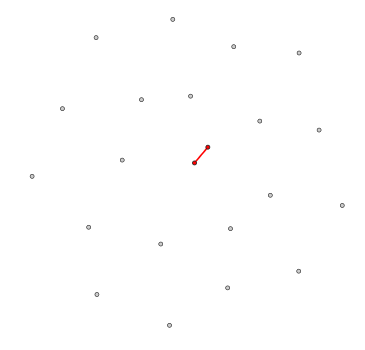
\includegraphics[width=0.92\textwidth]{figures/temporal/0.png}
        \caption{}
        \label{fig:temporal net A}
    \end{subfigure}
    \hfill
    \begin{subfigure}{0.3\textwidth}
        \centering
        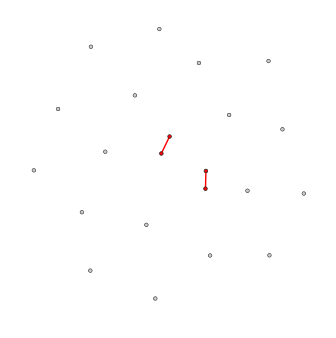
\includegraphics[width=0.92\textwidth]{figures/temporal/1.png}
        \caption{}
        \label{fig:temporal net B}
    \end{subfigure}
    \hfill
    \begin{subfigure}{0.3\textwidth}
        \centering
        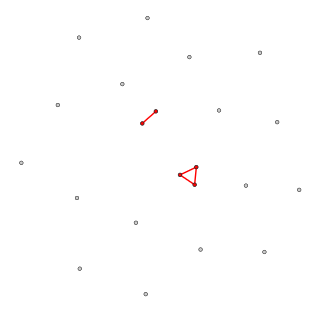
\includegraphics[width=0.92\textwidth]{figures/temporal/2.png}
        \caption{}
        \label{fig:temporal net C}
    \end{subfigure}
    \hfill
    \begin{subfigure}{0.3\textwidth}
        \centering
        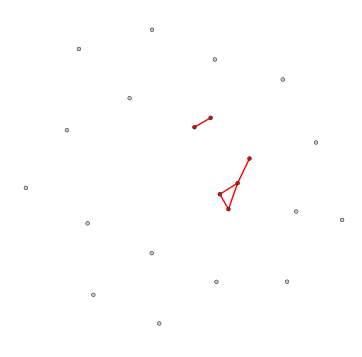
\includegraphics[width=0.92\textwidth]{figures/temporal/3.png}
        \caption{}
        \label{fig:temporal net D}
    \end{subfigure}
    \hfill
    \begin{subfigure}{0.3\textwidth}
        \centering
        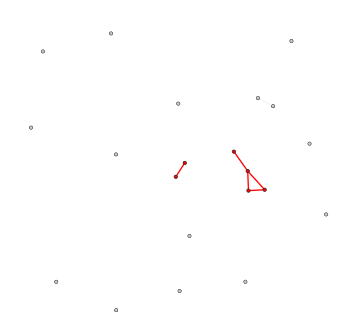
\includegraphics[width=0.92\textwidth]{figures/temporal/4.png}
        \caption{}
        \label{fig:temporal net E}
    \end{subfigure}
    \hfill
    \begin{subfigure}{0.3\textwidth}
        \centering
        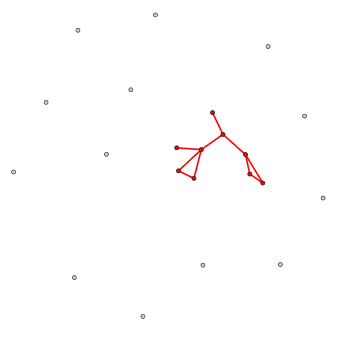
\includegraphics[width=0.92\textwidth]{figures/temporal/5.png}
        \caption{}
        \label{fig:temporal net F}
    \end{subfigure}
    \caption{Sequential snapshots of the \texttt{networkx} collaboration network with a moving time-window of 30 days and 7-day steps.}
    \label{fig:temporal net}
\end{figure}

Although a temporal network preserves the time aspect of the graph by the edges being tied to the time dimension of the graph, calculating network metrics like centrality on such networks is infeasible. Visualization also proves to be difficult in representations where animation is not possible. Therefore, we aggregate the bipartite network over a given timeframe into a static network. All nodes within the temporal net are preserved, and all directed edges are added to the network with the edge weight representing how many times that author edited the file. \\

\subsubsection{Static networks}
The generated static weighed bipartite network looses its time-varying component, but now we are able to manipulate and calculate complex statistics over it. Figure \ref{fig:bipartite} is an example of such a network. As a next step, we convert the the bipartite network into an authors' network by removing the nodes representing files. \\

\begin{figure}
    \centering
    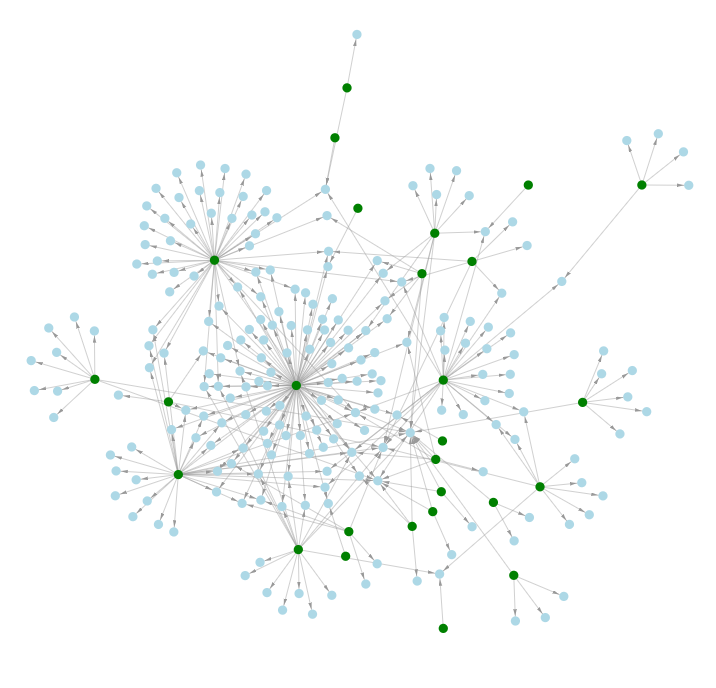
\includegraphics[width=0.65\textwidth]{figures/bipartite.png}
    \caption{A bipartite network of authors (green) and edited files (light blue) in the \texttt{pandas} project within the timeframe 31/01/2021 and 15/02/2021}
    \label{fig:bipartite}
\end{figure}

We have multiple methods to convert the directed and weighted bipartite network into a projection of authors. We could simply remove the files and connect each author, that worked on the same file, however, the end result would be an unweighted graph. This would falsely show, that all collaborations are weighed equally, which is clearly not the case, as multiple continuous edits on the same file from both parties should represent a stronger collaborative connection. Therefore, firstly we implement the Weighted One-Mode Projection (WOMP) method \cite{stramWeightedOneMode2017}, The WOMP method converts the bipartite network $G(A,F,E)$, where $E$ is the edge list containing tuples $(a_i,f_i,w_{ij})$, and $w_{ij} \in E$ is the weight between author $a_i \in A$ and file $f_i \in F$. With this notation, a weighted directed edge can be calculated for any $a_a, a_b \in A$ as follows:

\[ w_{ab}^{A \rightarrow A} = \sum_{j=1}^m \frac{w_{aj}}{W_a^F}, \]

where $W_a^F$ is the sum of all outgoing edge weights from author $a$ to all files $F$ denoted as $W_a^F = \sum_{i=1}^n w_{ai}$. This creates a bidirectional weighted collaboration network between authors $a_1$ and $a_2$, where the weight $w_{12}$ represents the relative collaboration effort of $a_1$ towards $a_2$ compared to all the other developers $a_1$ has collaborated with. Conseqently, every edge is in the rage $[0,1]$ in the resulting WOMP network. \\

A disadvantage of the WOMP method is, that the generated collaboration network is bidirectional, meaning if there was any common authored files between $a_1$ and $a_2$, then there will be both $w_{12}$ and $w_{21}$ connecting them. To simplify the network, we want to generate an authors network, where the edges are undirected. For this, we are using the weighted Jaccard method on the files-authors bipartite network:

\[ w_{ab} = \frac{\sum_{f \in F}min(f_a, f_b)}{\sum_{f \in F}max(f_a, f_b)}. \]

For each file $f$ that $a_1$ and $a_2$ authors touch, we sum up the minimum and maximum weights the authors have towards each file, then we divide the sum of minimums with the sum of maximums. This results in the undirected author-author network with edge weights in range $[0, 1]$. By default, this method removes isolated contributors, who do not collaborate with eachother, but are actively editing the files. We add these nodes manually. Figure \ref{fig:jaccard} shows the final author network. \\

\begin{figure}
    \centering
    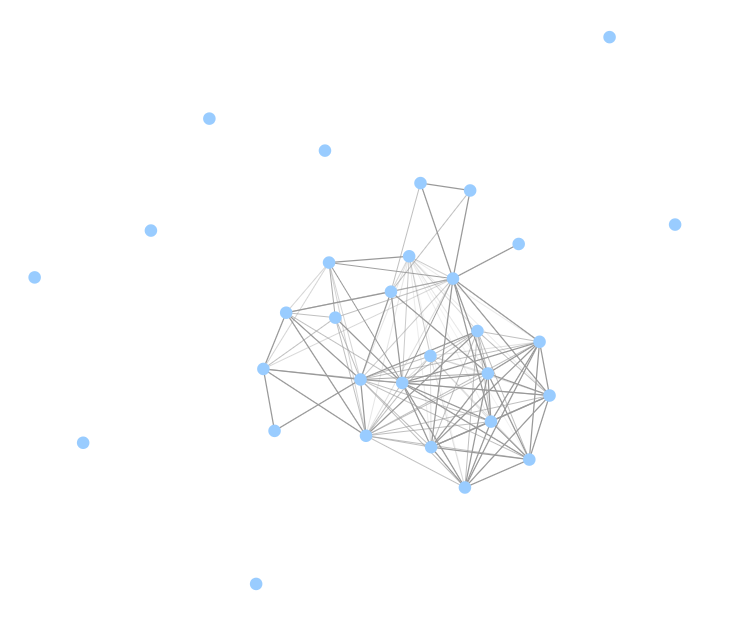
\includegraphics[width=0.9\textwidth]{figures/jaccard.png}
    \caption{Weighted Jaccard similarity collaboration network of \texttt{pandas} generated from the bipartite network in Figure \ref{fig:bipartite}.}
    \label{fig:jaccard}
\end{figure}

\subsection{Core and periphery, centralization}
A critical part of the OSS software projects is the existence of core and periphery developers. It has been observed, that in each FLOSS project there are a small number of developers, who provide the vast majority of development effort into the project. It has been also established, that the members of core developers do not change substantially during the project's lifecycle. However, there was no effort on whether there is a change in the collaboration pattern, especially before, during or after a major lifecycle event. Therefore, we make efforts identifying the core developer network to observe these changes. \\

\subsubsection{Degree centrality}

We use the degree centrality of each node (i.e. developer) to identify the core members. Degree centrality of a node is the fraction of all possible nodes it is connected to. We can calculate it by dividing the degree with $n-1$, where $n = |G|$ the number of nodes within the network. Since the core developers contribute the majority of commits and edits of the project, they are expected to be connected with more nodes. Joblin et. al. \cite{joblinClassifyingDevelopersCore2016, joblinEvolutionaryTrendsDeveloper2017} have also identified degree centrality as the best predictor of core developers. In cases, where binary classification of core or periphery is needed, we assign developers to the core network if their degree centrality score is in the top 20th percentile, otherwise they are considered as periphery. We also take note, that this method does not consider the weighted edges, only the number of edges (degree) a node has. Although this method could be refined to consider the node degree weighted with the edges, we argue that this could lead to invalidity. In case of two developers, who only contributed to one file, they will be represented with a strong connection and would receive a high weighted degree value, whereas a core contributor, who edits many files, can have many weak connections but these might not add up to one strong connection of the two isolated developers when weighted with the edge weights. It is clear, that a developer with many connections, regardless of the strength of the collaboration, should be considered core. Figure \ref{fig:degree centrality} shows two examples for degree centrality within a collaboration network. In the figure, darker colors represent a higher degree centrality value. The  highlighted nodes are in the highest 20th percentile of degree centrality, classifying as members of the core developers. We can observe in both one-month periods, that \texttt{pandas} is much more decentralized, whereas \texttt{curl} is largely dependent on one developer.\\

\begin{figure}
    \centering
    \begin{subfigure}{0.49\textwidth}
        \centering
        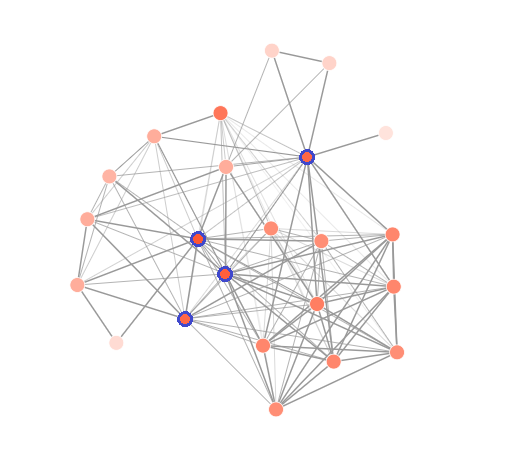
\includegraphics[width=0.98\textwidth]{figures/degree_centrality.png}
        \caption{Pandas}
        \label{fig:centrality a}
    \end{subfigure}
    \hfill
    \begin{subfigure}{0.49\textwidth}
        \centering
        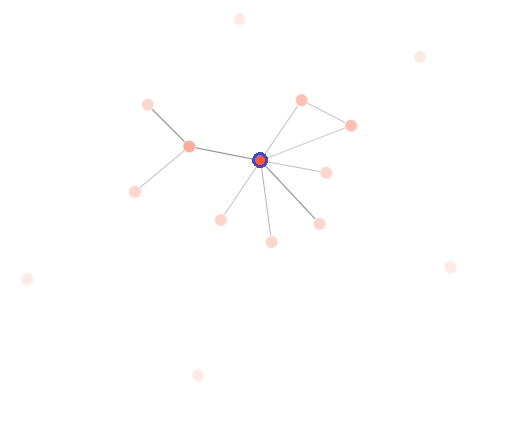
\includegraphics[width=0.98\textwidth]{figures/degree_centrality_curl.png}
        \caption{Curl}
        \label{fig:centrality b}
    \end{subfigure}
    \caption{Degree centrality within the \texttt{pandas} and \texttt{curl} projects' collaboration networks. }
    \label{fig:degree centrality}
\end{figure}

\subsubsection{Degree centralization}

The degree \textit{centrality} can be calculated for every node, however, through our analysis we would also like to measue a global \textit{centralization} metric, which is applicable to the whole network. As suggested by Crowston and Howison \cite{crowstonHierarchyCentralizationFree2006}, we calculate the degree \textit{centralization} by summing the differences between the maximum and each node's degree \textit{centrality}. 

\[ C_D(A) = \frac{\sum_{i=1}^n(C_d(a*)-C_d(a_i))}{H}, \]

where $C_d(a)$ is the degree \textit{centrality} of an author $a$, $a*$ is the author with the highest degree \textit{centrality} value, and $n$ is the number of authors in the collaboration network $A$. The value $H$ is for normalizing the sum by dividing by the theoretical maximum \textit{centralization}. Since the \textit{centrality} values are already in the range $[0, 1]$, we only need to normalize for the network's size. We get the highest centrality score with a star graph, where each node is only connected to a single central node, which has exactly one edge to all other nodes. The central node has a centrality of 1 in this case, whereas all the other $n-1$ nodes have $C_d(a) = \frac{1}{n-1}$. This means that in case of a star graph:

\[ H = (n-1) (1-\frac{1}{n-1}) = n-2. \]

Within certain timeframes, when a project is inactive, it could happen, that the network contains 2 nodes or less. We define $C_D(A) = 0$ if $|A| = n <=2$. The resulting output will always have a value in $[0, 1]$, where 1 means a completely centralized network (star graph) and 0 means a completely decentralized network. It is important to emphasize that a centralization score of 0 does not necessarily mean that there is no collaboration and every developer is isolated. Rather it means that each developer is co-authoring with just as many authors, as the others do. \\

% - Gini coefficient

% - \cite{klugUnderstandingGroupDynamics}

\subsubsection{Clustering coefficient}

While centralization helps us describe the centralness of the network and how much it is centered around a single, or a small number of developers, it does not help us describing the structure of the network in more detail. Our goal is to gain an understanding of also the modularity of our network, meaning how much developers tend to cluster together \cite{joblinEvolutionaryTrendsDeveloper2017}. We expect that authors form smaller clusters, which are more tightly connected together, and these clusters have somewhat weaker ties to other clusters. This builds on the assumption that the social network of the software follows the modules which build up the software itself, thus authors of a specific function should also cluster together within the network \cite{conwayHowCommitteesInvent1968, joblinEvolutionaryTrendsDeveloper2017}. To measure this "clusteredness", we calculate the \textit{local clustering coefficient} for each node. \\

\begin{figure}
    \centering
    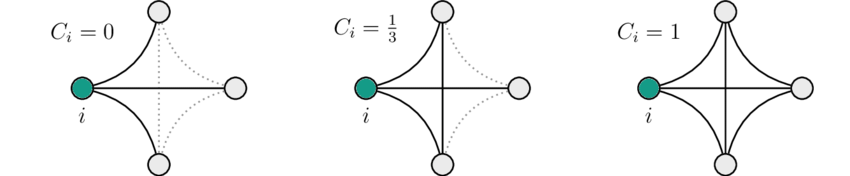
\includegraphics[width=1\textwidth]{figures/loc_clust_coeff.png}
    \caption{The local clustering coefficient demonstrated on an unweighted network of 4 vertices \cite{jedrzejewskiRoleComplexNetworks2016}.}
    \label{fig:loc clust coeff}
\end{figure}

The \textit{local clustering coefficient} quantifies on a scale $[0, 1]$ how likely it is that a node's neighbours are also neighbours. We use the number of how many triangles (also called clique, triplet) is every node a part of. This is illustrated for unweighted networks on Figure \ref{fig:loc clust coeff} with the formula:

\[ C_i = \frac{2T(i)}{deg(i)(deg(i)-1)}, \]

where $T(i)$ is the number of triangles through node $i$ and $deg(i)$ is the degree of i. However, in a weighted network we also have to consider the edge weights, since it is easy to see that a clustering coefficient of 1 with also the maximum weighted edges in a triplet does not represent the same clustering as being connected with a weak links. We expect weaker links connecting larger clusters, whereas stronger links within each cluster. Therefore, we use geometric averaging of the subgraph edge weights (as implemented by the \texttt{networkx}\footnote{\url{https://networkx.org/documentation/stable/reference/algorithms/generated/networkx.algorithms.cluster.clustering.html}} library \cite{onnelaIntensityCoherenceMotifs2005}):

\[ c_i = \frac{\sum_{jk}(\hat{w}_{ij}\hat{w}_{ik}\hat{w}_{jk})^{1/3}}{deg(i)(deg(i)-1)}. \]

The $\hat{w}_{ij}$ represents the normalized weight of edge $e_{ij}$ over the maximum weight in the network. \\

\subsubsection{Hierarchy}
The degree centrality and the clustering coefficient are in themselves able to express meaningful aspects of the developer social network, however, by combining the two metrics, we can also assess how hierarchical the network is. In a scale-free social hierarchical network (such as the collaboration network), nodes tend to cluster around a single or a few hubs, which are more likely to have weak connections to other hubs \cite{ravaszHierarchicalOrganizationComplex2003, joblinEvolutionaryTrendsDeveloper2017}. The nodes within these formed groups are relatively stronger than the connections connecting the hubs, but they are less likely to connect to nodes outside of their group. Therefore in a hierarchical network, the hubs have a high degree number and a low clustering coefficient, whereas the group members clustering around the hubs have a high clustering coefficient, but low degree numbers. \\

We can visualize the degree of hierarchy by plotting each node's  clustering coefficient against the number of degrees, shown in Figure \ref{fig:hierarchy}. In hierarchical networks, the plotted linear regression trendline will decrease steeply, as there is a negative correlation between the degree and clustering coefficient. In networks, where this cannot be observed, the trendline stays flat, meaning these two metrics are independent from eachother and the structure is not hierarchical. To measure the hierarchical level numerically within a network, we take the trendline's slope, which is $\beta_1$ in the $y=\beta_1x + \beta_0$ general linear regression equation. \\

\begin{figure}
    \centering
    \begin{subfigure}{0.49\textwidth}
        \centering
        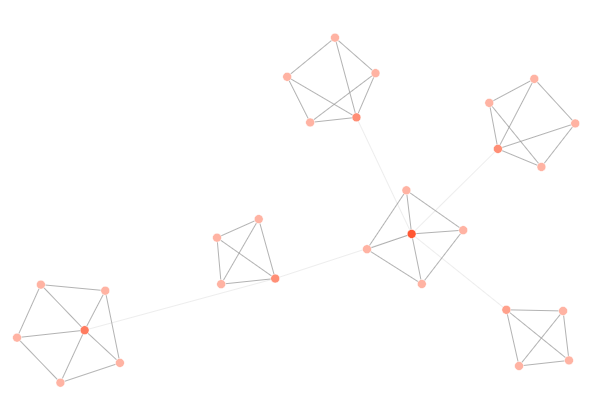
\includegraphics[width=0.98\textwidth]{figures/hierarchical.png}
        \caption{Highly hierarchical network}
        \label{fig:hierarchical}
    \end{subfigure}
    \hfill
    \begin{subfigure}{0.49\textwidth}
        \centering
        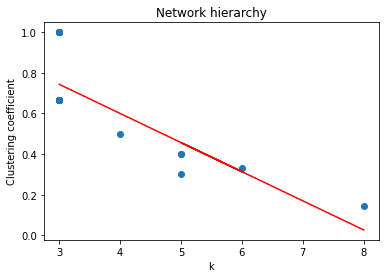
\includegraphics[width=0.98\textwidth]{figures/hierarchy_plot.png}
        \caption{Network hierarchy}
        \label{fig:hierarchy plot}
    \end{subfigure}
    \caption{Hierarchical network and its corresponding degree number vs clustering coefficient plot.}
    \label{fig:hierarchy}
\end{figure}

In every network isolated authors can be observed, who are only working on files that noone else has edited (in the given timeframe). These nodes can skew the hierarchy score, because an isolated node's degree and clustering coefficient are by definition 0, which disproportionately makes the trendline much flatter. Therefore, we remove the isolated nodes from the network. If the network only contains isolated nodes, and there is no linear regression to be calculated, we set the hierarchy value to 0.

\subsection{Project measures}

One of our assuptions is that the collaboration network structure changes depending on the project's lifecycle. In order to discover cause and effect relationships between the network structure and project lifecycle, we gather basic project metrics to pinpoint the time and date of events, as well as the effort required within the project. We achieve this by gathering the dates of each release, and the quality and relative stress is measured by the issues within the project (create and close times).

\subsubsection{Release and release measures}

To measure the network changes around releases, first we collect the list of releases for the given project. Our goal is to gather the version number of each release, as well as the dates they were released. There are two relevant APIs regarding the release version numbers: GitHub releases and Git tags. Tags are marked and annotated commits supported by Git, therefore other projects, that are not on GitHub can also have tags. \textit{Tags} are most commonly used to mark new release versions, but they can also be used to annotate other information, such as release editions or milestones. On the other hand, a \textit{Release} is a high-level GitHub concept, which allows the project organizers to announce Git tags as project releases by adding a version number, release notes and binary artifacts \cite{olsonReleaseYourSoftware2013}. A commit, that represents a new GitHub release, must be tagged, but a tagged commit does not necessarily need to be a new GitHub release. \\

\begin{figure}
    \centering
    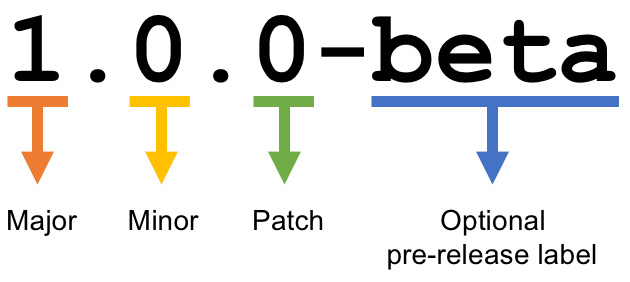
\includegraphics[width=0.5\textwidth]{figures/semantic-versioning.png}
    \caption{Semantic versioning. Figure source: \cite{SemanticVersioningUT2018}.}
    \label{fig:semver}
\end{figure}

Throughout our analysis, we use the tags as indicators of a new release, because there could be new versions of a software, that are not released publicly, and therefore do not have a GitHub release. Furthermore, GitHub only announced the Releases workflow in 2013, when the release versioning by Git tags was already a common practice. This means, that releases before 2013 can only be analysed via the repository tags. \\

Most large-scale OSS proejcts follow the semantic versioning convention, but only to a certain extent. The majority of tags follow the major-minor-patch (also known as breaking-feature-fix) semantic version naming convention in the format of X.Y.Z, where X is the major number, Y is the minor number, and Z is the patch number \cite{preston-wernerSemanticVersioning}. At the end, optionally pre-release and build data can be marked, for example: \textit{1.11.6-pre}. The major number signifies an API-breaking change compared to the previous release, meaning backwards compatibility is not guaranteed for depending applications. Minor releases add new features, but compatibility is ensured with the older version. Patch releases usually handle bugs and security updates within the package. \\

During the network analysis, we expect the network measures to change around a release, but it is also expected, that a larger release, that required more collaboration, will have a greater impact, while smaller changes have smaller or no impact at all. The issue with the semantic versioning and release names is that there are no constraints, which would enforce a strict version naming, and it is entirely up to the developers to set the tag names. This leads to inconveniences when measuring collaboration effort through release version number, because a patch might require more collaboration effort than a minor release, and a minor release within one project could require significantly more teamwork than in another. Furthermore, tag names can be inconsistent, and there could be version numbers, that do not adhere to the major-minor-patch naming convention at all (e.g. test releases, or releases like 'latest-release-v11'). The possibility to add extra information at the end of tag names, like \texttt{-beta} or \texttt{rc} further complicates tracking the collaboration effort, because the majority of collaboration effort might happen before the \texttt{rc} version, or it might happen after it. As it can also be seen in Table \ref{tab:releases}, the \texttt{v0.14.0rc1} tag contains more modifications than the final \texttt{v0.14.0} version, whereas the \texttt{v1.2.0rc0} only contains a small fraction of modifications compared to \texttt{v1.2.0}. \\

\begin{table}
    \centering
    \resizebox{\textwidth}{!}{%
        \begin{tabular}{| c | c | c | c | c | c | c | c | c |}
            \hline
            \textbf{Index} & \textbf{Name} & \textbf{Tag name} & \textbf{Created} & \textbf{Type} & \textbf{Modifications} & \textbf{Lines added} & \textbf{Lines removed} & \textbf{Total change} \\
            \hline \hline
            0 & Pandas v0.13.0 & v0.13.0 & 2013-12-30 17:02:51 & unknown & 20031 & 1.665357e+09 & 1.624343e+09 & 3.289700e+09 \\
            1 & Pandas v0.13.1 & v0.13.1 & 2014-02-03 04:52:01 & patch & 836 & 2.231875e+06 & 2.349833e+06 & 4.581708e+06 \\
            2 & Pandas v0.14rc1 & v0.14.0rc1 & 2014-05-16 22:28:09 & minor & 1861 & 2.251189e+07 & 2.050846e+07 & 4.302035e+07 \\
            3 & v0.14.0 final & v0.14.0 & 2014-05-30 11:47:40 & unknown & 318 & 3.220804e+06 & 5.314470e+05 & 3.752251e+06 \\
            4 & v0.14.1 final & v0.14.1 & 2014-07-10 23:46:19 & patch & 720 & 1.660133e+06 & 3.796690e+05 & 2.039802e+06 \\
            5 & v0.15.0 Pre-release & v0.15pre & 2014-09-07 12:52:01 & unknown & 826 & 1.028779e+07 & 2.458664e+06 & 1.274645e+07 \\
            \dots & \dots & \dots & \dots & \dots & \dots & \dots & \dots & \dots\\
            66 & Pandas 1.1.5 & v1.1.5 & 2020-12-07 11:42:10 & patch & 2167 & 4.251057e+06 & 4.611365e+06 & 8.862422e+06 \\
            67 & Pandas 1.2.0rc0 & v1.2.0rc0 & 2020-12-08 12:31:44 & minor & 41 & 1.060500e+04 & 8.850000e+02 & 1.149000e+04 \\
            68 & Pandas 1.2.0 & v1.2.0 & 2020-12-26 13:47:00 & unknown & 683 & 5.782570e+05 & 2.989310e+05 & 8.771880e+05 \\
            69 & Pandas 1.2.1 & v1.2.1 & 2021-01-20 11:21:02 & patch & 1306 & 1.864636e+07 & 9.228629e+07 & 1.109326e+08 \\
            70 & Pandas 1.2.2 & v1.2.2 & 2021-02-09 10:55:19 & patch & 844 & 6.783283e+06 & 1.827142e+07 & 2.505470e+07 \\
            71 & Pandas 1.2.3 & v1.2.3 & 2021-03-02 09:43:36 & patch & 959 & 1.002189e+07 & 5.783745e+06 & 1.580563e+07\\
            72 & Pandas 1.2.4 & v1.2.4 & 2021-04-12 15:59:13 & patch & 289 & 3.402820e+05 & 1.704960e+05 & 5.107780e+05\\
            \hline
        \end{tabular}} \\
    \caption{Releases collected information.}
    \label{tab:releases}
\end{table}

In order to have a more fine-grained measure of how much effort a release required (besides the semantic versioning), we measure the number of lines added and lines removed in that release. This is calculated by adding up each commit's 'total lines added' and 'total lines removed', which was authored after the previous release but up to and including the current release tag's commit. The total change of lines for a release is simply the sum of lines added and lines removed, which are provided by the \texttt{git2net} miner. The miner also provides the number of modifications for each commit. A modification is a section of the source code modified, which can mean multiple lines added and deleted at the same part of the document. For example, if a new function is added to the project, which requires 20 new lines and removes 2 lines (e.g. empty space that was there before), then it will be considered as 1 modification, but 22 total line change. Changes to binary files are due to generated artifacts, which do not carry any collaboration effort, therefore they are excluded, and commits, that do not have a hash are also removed. \\

The release type contains the semantic version of the release, which was gathered from the tag name with a Regular Expression matching the conventional versioning X.Y.Z. We also capture the version number in tags, that contain additional notations such as \texttt{beta} or \texttt{rc}, then we compare the current release to the previous to identify whether the release is a major, minor or patch release. When the found version numbers in the previous and in the current release are the same, we leave that as unknown, as this is mostly the case in pre-releases. The first release doesn't have a preceeding tag, therefore we consider every modification before the tag as part of the release. This leads to the first tag seeming to have significantly more edits than the rest of the releases, whereas in fact this is just the result of not tracking from the beginning (see example in Table \ref{tab:releases}). Therefore, in our analyses we remove the first release, as this would lead to falsely weighing the network results. \\



\subsubsection{Project issues and measures}

To measure the productivity within the project, we collect some basic information regarding the GitHub issues. Issues keep track of bugs, beatures and tasks, contributors can comment and discuss the task at hand within an issue, and it can be assigned to users and milestones can be set. We collect the following information of issues:

\begin{itemize}
    \item Issue title
    \item Issue number
    \item Created at
    \item Closed at
    \item Open for
    \item Bug or feature
\end{itemize}

The \textit{issue title} is a short description of the issue. Most projects create their own convention of naming and tagging issues, for example each issue starts with a 3-letter abbreviation of a category, e.g. \texttt{BUG} or \texttt{DOC}. \textit{Issue number} is a unique number for each issue, that is increased sequentially. \textit{Created at} is the date and time of the issue being created, and \textit{closed at} is the time when it was closed. If the issue was still open on the day of data mining (May 9 2021), this field is empty. The \textit{open for} field is the difference between the \textit{closed at} and \textit{created at} dates, or it is empty if the issue was never closed. \\

\begin{figure}
    \centering
    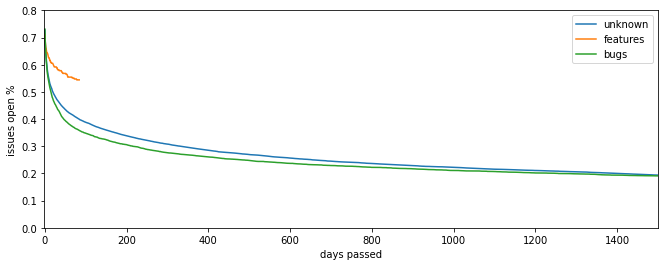
\includegraphics[width=0.9\textwidth]{figures/issues_open.png}
    \caption{Survival curves of the \texttt{pandas} library.}
    \label{fig:survival}
\end{figure}

The last measure is \textit{bug or feature}. Because issues can cover a wide range of possible topics, from discussions to performance, it is worth categorizing them to analyse the differences. However, categorization in practice proves to be difficult due to the different conventions each project uses, and because GitHub does not apply any constraints to the text of the title. We are searching for specific keywords in the \textit{issue title} to categorize each issue into either a bug or a feature. We also drop some of the words from the text, because they would give us 'false positive' matches. If keywords for both or neither categories are found, the issue is marked as unknown. The dropped words, as well as the bug and feature keywords can be seen in Table \ref{tab:keywords} Although this simple method can already classify 10-15 percent of issues, it would require extensive manual effort to further improve this ratio. In future research, sentiment analysis of issue titles and issue descriptions could achieve much higher percentages. \\

Statistics for issues like average close time also prove to be difficult, because there are continuously open issues, which inevitably leads to the fact that a large portion of issues were still open and continue to be open. For these issues, we cannot know the issue close time, and if we try to calculate global measures by aggregating all (or portion) of issues, we have to consider the \textit{survival bias} \cite{jarczykSurgicalTeamsGitHub2018}. Figure \ref{fig:survival} shows the issues survival curve of the \texttt{pandas} library. It is clearly visible, that a large portion (20 percent) of issues are not closed, and if we left them out of aggregate values such as average open time, our data will be skewed. Nevertheless, we can see in the example, that the categorization of issues makes a difference, as bugs get closed a bit earlier than an average (unknown) issue, because after the same amount of days passign for both categories, more bugs tend to be closed in this example. In contrast, features have a high life expectancy, as they are more likely to be still open than a bug, if the same number of days pass. The reason could be that features take longer to develop and plan than bugs, which is consistent with the findings of Jarczky et. al. \cite{jarczykSurgicalTeamsGitHub2018}. \\

\begin{table}
    \centering
        \begin{tabular}{| c | c | c |}
            \hline
            \textbf{Drop words} & \textbf{Bug keywords} & \textbf{Feature keywords} \\
            \hline \hline
            debug & bug & feature \\
            debugger & defect & enhancement \\
            debugging & incorrect & improvement \\
             & unexpected & suggestion \\
             & error & wishlist \\
             & missing & wish list \\
             & warning & \\
             & problem & \\
            \hline
        \end{tabular}
    \caption{Keywords and drop words for \textit{bug} and \textit{feature} categorization.}
    \label{tab:keywords}
\end{table}


\section{Collaboration pattern analysis}
The focus of our analysis is how the collaboration network of FLOSS projects changes during their lifecycle. Moreover, we are also interested in the cause of the changes, rather than just observing the changes. Therefore we determined two types of events, that we want to observe in order to see the effects on the collaboration. The events during a project's lifecycle can be one of two types: regular or irregular event. Regular events repeat over time with roughly the same time passing between events. This can be a holiday season (e.g. summer holidays or at the end of the year) or regular software releases. In our research, we will focus on only the software releases, and we suggest the analysis of collaboration and seasonality as a future research topic. In contrast to releases, which are usually well documented and easily discoverable when exactly they were released, irregular events are harder to discover, as these do not necessarily stem from within the developer community, but from external sources. Examples could be a supporting company's organizational restructuring, the sudden increase of work from home during the COVID pandemic, or mass layoffs within the support team. In our analysis, we will mainly focus on layoff events, because of our expectation that this will have the largest effect on collaboration. Usually when a company develops an open-source software, the company relies on the external community of the project, but the core developers are mainly from the company. Therefore, when a company officially pulls out from further development, this results in the removal of most core developers in a short amount of time. Our main goal is to identify how this affects the collaboration network, how the network restructures itself, or if any restructuring occurs at all. \\

As a first step, we conduct a qualitative analysis on a number of hand-picked repositories to observe the network statistics in detail and to identify cause and effect relationships. In order to avoid bias when selecting repositories, we choose projects based on a variety of factors:

\begin{itemize}
    \item \textit{Project size:} We define the project's size as small, if it has less than 100 contributors, medium sized if the number of collaborators are between 100 and 500, and large if it has more than 500 collaborators.
    \item \textit{Centralization:} Although it is hard ot measure how decentralized a project is, based on the literature review, very large projects tend to be decentralized. For now, we consider those projects centralized, which have been identified as centralized in the current state-of-the-art literature. 
    \item \textit{Event occurrences:} Whether there is a regular release cycle within the project or not based on the release dates, or if there are known and confirmed cases of unexpected layoff events.
\end{itemize}

Based on these criteria, we try to select a wide variety of projects, so that each type (small, medium or large size, centralized or decentralized, regular or irregular or abandoned projects) has at least one example. We acknowledge the fact that this inclusion criteria leaves room for selection bias, as an observed correlation between events and the network in one project might not hold true for all projects. However, later we confirm our hypotheses with a quantitative analysis. \\

\subsection{Project selection and descriptions}

All together we choose 8 projects to analyse, these can be seen in Table \ref{tab:projects}. Due to the repository miner's limitation, we are only considering projects maintained on GitHub. The \texttt{pandas} and \texttt{numpy} repositories are well-known and popular data science tools for data manipulation in Python. They are very similar in size and popularity, both with a huge base of collaborators. Since also the number of issues are really high, our expectation is that these projects are highly decentralized, where the developers mainly work on their own parts of the project. They also have fairly regular release cycles, with a minor release in every 5-6 months. \\

\texttt{Networkx} and \texttt{seaborn} are both middle-sized repositories based on the number of contributors, and they are both used for data visualization and statistical analysis in Python-based software, but \texttt{networkx} visualizes networks and their related statistics, while \texttt{seaborn} creates various plot images. Each release date follows the previous with 4 to 10 months, which means their releases are not as regular as the first two repositories. \\

The project \texttt{curl} is an example for a highly centralized project, as its source code is famously maintained by a single developer \cite{crowstonHierarchyCentralizationFree2006}. Based on the number of contributors, it is a medium-sized project, although the number of commits are much higher than \texttt{networkx} or \texttt{seaborn}. Being the oldest project from the selection might contribute to the large number of commits. \\

\begin{table}
    \centering
    \resizebox{0.85\textwidth}{!}{%
        \begin{tabular}{| c | c | c | c | c | c | c |}
            \hline
            \textbf{Name} & \textbf{Contributors} & \textbf{Size} & \textbf{Commits} & \textbf{Stars} & \textbf{Issues} & \textbf{First release}\\
            \hline \hline
            pandas & 2333 & large & 26792 & 29700 & 3518 & Feb 20, 2011 \\
            numpy & 1135 & large & 26392 & 17200 & 2030 & Jan 5, 2002 \\
            networkx & 469 & medium & 6470 & 9100 & 166 & Jul 17, 2005 \\
            seaborn & 140 & medium & 2780 & 8400 & 82 & Oct 28, 2013 \\
            curl & 701 & medium & 27159 & 20600 & 27 & Mar 14, 2000 \\
            servo & 1101 & large & 44084 & 19600 & 3305 & May 22, 2017 \\
            wasmtime & 243 & medium & 8334 & 5200 & 341 & Oct 18, 2016\\
            py-junos-eznc & 69 & small & 2486 & 583 & 76 & Nov 3, 2013\\
            \hline
        \end{tabular}}
        \caption{Collaboration analysis projects and basic statistics.}
        \label{tab:projects}
\end{table}

\texttt{Servo} and \texttt{wasmtime} are both based on the Rust programming language, and they are both used for web applications: \texttt{Servo} is a browser engine, whereas \texttt{wasmtime} is a runtime environment for WebAssembly. Both projects were led by Mozilla and maintained in an open-source environment. The Rust developer team was heavily affected by the Mozilla layoffs on January 15\textsuperscript{th}, 2020 and August 11\textsuperscript{th}, 2020 \cite{MozillaLays70,kastrenakesMozillaLaying2502020}, with the second round of layoffs affecting all Rust employees. The \texttt{py-junos-eznc} project is considered small, since it has less than 100 contributors, and it is a Python-based library for automatizing devbices running on Juno OS. On May 27\textsuperscript{th}, 2020, the sponsoring company Juniper Networks laid off its entire open source developers \cite{FarewellJuniperNetworks2020}. These three projects will be the main focus of analysing unexpected, one-time events and layoffs, where we will take a close look at the network statistics around the mentioned dates. \\ 

To reliably compare the projects, we have to consider only a slice of each project, so all of them are compared within the same time period. We take a 3-year period from 2018 to the end of 2020. All projects had their first release before this period, which means this should filter out the initial irregular activities, such as creating directories and restructuring. \\

\subsection{Commits analysis}

For the selected period, we check the number of commits in each project as a first step. This can be seen on Figure \ref{fig:commits}. To smooth out the stacked area plot, we summed up the number of commits in every 28 days. Purposefully a multiple of 7 was chosen in order to even out the possible irregularities caused by the weekdays and weekends. We can see that all projects are active, with varying magnitude of commits generated each month. The number of commits are consistent with the size of the project, but we can also see that the number of contributors and the number of commits are not completely dependend on eachother, as \texttt{servo} consistently receives more commits than the other large repositories, despite the fact that it has the same number of contributors as \texttt{numpy} and half as many as \texttt{pandas}. Our assumption is, that this is highly dependent on the type of software being developed, the used programming language(s) and on other project-specific properties. \\

There is a noticeable decrease in the number of commits to \texttt{servo} at the time of the layoffs (August 2020), which signals that the project could have been affected. This cannot be observed for \texttt{wasmtime}. We do not see any evidence of reoccurring trends within the number of commits, e.g. decreased activity during holiday season. There is a reduction in all repositories at the end of 2018, but this is contradicted by a spike in the number of commits at the end of 2019. However, we cannot rule out any periodicity, because this could be hidden due to the 28-day aggregation. \\

\begin{figure}
    \centering
    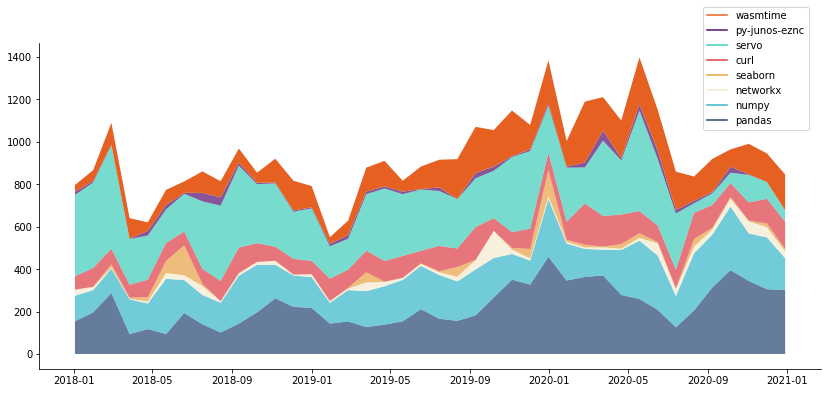
\includegraphics[width=\textwidth]{figures/commits.png}
    \caption{Number of commits in each month.}
    \label{fig:commits}
\end{figure}

\subsection{Releases}
As a next step, we take a look at the regular lifecycle events, which are the releases in the open source projects. We generate the collaboration networks for the same time period (between 2018 and 2020) and contrast them with the time of releases. \\

The issue with generating the collaboration network is the time aspect: we cannot observe any collaboration network if we take a single point in time and create the network for a given timestamp, as this will only contain a handful of connections, who authored an edit in the same file at the exact same time. Therefore, we need to aggregate the edits and commits over time, which requires us to use a time window to scan through the observed time period, and for each step, we generate a snapshot of the network. The first parameter is the time window length and the second is the step size. By choosing a large time window, we observe more connetion within the generated graph, but with a too large value, the network becomes too much grouped together, with almost every node connecting to almost all other nodes. By setting this value too low, the result is a disconnected network. The step size determines how often we take a screenshot of the network for the time window. By default, we use one-day steps, but sometimes this results in too radical changes. Therefore in some cases we use a 7-day or a 28-day step value to smooth out the curves. However, a too high step value can obscure the changes we want to observe.\\

\subsubsection{Release regularity}

\begin{itemize}
    \item time window
    % - Time window scanning over time
    % - parameters: delta, interval, from, to
    % - size of the project matters
    % - activity determines the scale (less activity = small interval (week), vice versa)
    
    % - The efficiency of a project’s workflow (measured by the percentagesof issues assigned to specific developers). \cite{jarczykSurgicalTeamsGitHub2018}
    
    \item network stats plots (with major-minor-patch)
    \item results (e.g. degree centrality, clustering coeff, hierarchy) for each project
\end{itemize}
\subsection{External events}
\subsection{Observed projects and events}
% - which projects (Servo, pandas, numpy, networkx, seaborn, wasmtime, ruptures (?))
% - expected: Big releases
% - unexpected: layoffs
\subsection{SNA metrics analysis}
\subsubsection{K-cores}
Besides taking the 20th percentile of the top clustering coefficients to identify the number of core developers in the network, we .... \cite{batageljAlgorithmCoresDecomposition2003}
% - 20th percentile of k-core nodes
% - alternative to identifying the core members
%....
\subsection{Results}
%....


% (\item Automatic event recognition)
%     (\item Event detection implementation (ruptures))
%     (\item Collaboration network change detection)
\section{Quantitative analysis of projects during crunch time}
\subsection{Collaboration network changes}
\subsection{Prediction of outcome based on collaboration changes}

\section{Discussion and results}
\section{Conclusion and future work}
